\documentclass[tikz,border=12pt]{standalone}
% Compile each standalone figure from its example subdirectory.
% Shared visual language for standalone EMT block diagrams.
\usepackage{amsmath}
\usetikzlibrary{arrows.meta,backgrounds,calc,fit,positioning}

\tikzset{
    emt diagram/.style = {>={Stealth[length=2.4mm]}},
    line/.style        = {semithick, rounded corners=6pt},
    block/.style       = {draw, semithick, fill=white,
                          minimum height=1cm, minimum width=2.3cm},
    hblock/.style      = {block, minimum width=2.24cm, minimum height=1.3cm},
    vblock/.style      = {block, minimum width=1.3cm, minimum height=2.24cm},
    sum/.style         = {draw, semithick, fill=white, circle,
                          inner sep=2.6pt},
    signal/.style      = {circle, fill, inner sep=1.4pt,
                          label distance=3pt},
    sig/.style         = {font=\small},
    pm/.style          = {font=\scriptsize},
    wire jump/.style   = {line,
                          preaction={draw=white, line width=3pt,
                                     line cap=round}},
    enclosure/.style   = {draw, dashed, semithick, rounded corners=4pt},
    operator enclosure/.style = {enclosure, inner xsep=7mm, inner ysep=6mm}
}


\definecolor{externalBusBlue}{HTML}{007AFF}
\definecolor{internalBusRed}{HTML}{D64545}

\tikzset{
    partition/.style = {enclosure, solid},
    partition group/.style = {enclosure},
    external reference/.style = {line, dashed, draw=black},
    physical branch/.style = {line, solid, draw=black!45},
    external bus/.style = {signal, fill=externalBusBlue},
    internal bus/.style = {signal, fill=internalBusRed},
    external bus label/.style = {sig, text=externalBusBlue, fill=white, inner sep=1pt},
    internal bus label/.style = {sig, text=internalBusRed},
    partition label/.style = {sig, fill=white, inner sep=2pt}
}


% Membership of the buses in the TenGen integration tests.
% The weak branch 5--6 belongs to A; bus 6 is shared with B.
\def\diagramScale{1}

\begin{document}
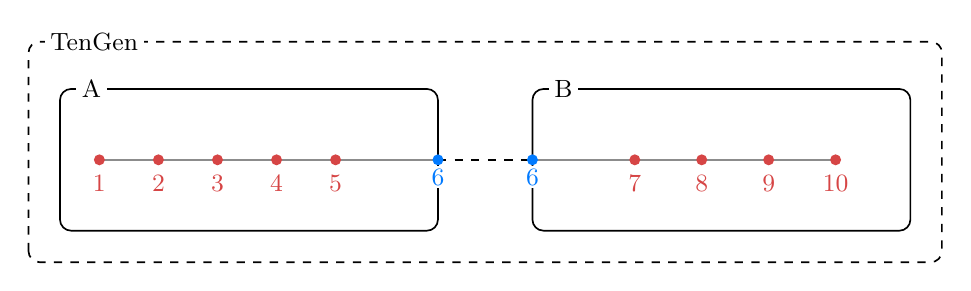
\begin{tikzpicture}[emt diagram, scale=\diagramScale, transform shape]
\draw[partition group] (-0.4, -0.4) rectangle (11.2, 2.4);
\node[partition label, anchor=west] at (-0.2, 2.4) {TenGen};
\draw[partition] (0, 0) rectangle (4.8, 1.8);
\node[partition label, anchor=west] at (0.2, 1.8) {A};
\draw[partition] (6, 0) rectangle (10.8, 1.8);
\node[partition label, anchor=west] at (6.2, 1.8) {B};

% Copies of the same bus; this connector is not the physical branch 5--6.
\draw[external reference] (4.8, 0.9) -- (6, 0.9);
% Physical branches 1--2--3--4--5--6 in A and 6--7--8--9--10 in B.
\draw[physical branch] (0.5, 0.9) -- (1.25, 0.9) -- (2, 0.9)
    -- (2.75, 0.9) -- (3.5, 0.9) -- (4.8, 0.9);
\draw[physical branch] (6, 0.9) -- (7.3, 0.9) -- (8.15, 0.9)
    -- (9, 0.9) -- (9.85, 0.9);
\foreach \bus/\x in {1/0.5,2/1.25,3/2,4/2.75,5/3.5}
    \node[internal bus, label={[internal bus label]below:$\bus$}] at (\x, 0.9) {};
\foreach \bus/\x in {7/7.3,8/8.15,9/9,10/9.85}
    \node[internal bus, label={[internal bus label]below:$\bus$}] at (\x, 0.9) {};
\node[external bus, label={[external bus label]below:$6$}] (bus6-A) at (4.8, 0.9) {};
\node[external bus, label={[external bus label]below:$6$}] (bus6-B) at (6, 0.9) {};
\end{tikzpicture}
\end{document}
